
\subsection{Cosmolog\'ia}

\begin{tikzpicture}[]
    % node definitions
    \node (s1) at (0, 0) {};
    \node (s2) at (1, 0) {};
    \node (s3) at (2, 0) {};
    \node (s4) at (3, 0) {};
    \node (s5) at (4, 0) {};
    % sketch
    \draw [test={1pt}{c1}{c2}, thick] (s1.center) to (s2.center);
    \draw [test={1pt}{c2}{c3}, thick] (s2.center) to (s3.center);
    \draw [test={1pt}{c3}{c4}, thick] (s3.center) to (s4.center);
    \draw [test={1pt}{c4}{c5}, thick] (s4.center) to (s5.center);
\end{tikzpicture}

La imagen que tenemos del Universo en el que vivimos ha estado fuertemente influida por dos \underline{observaciones} independientes:
\begin{itemize}
 \item La detección - inicialmente realizada por Arno Penzias y
Robert Woodrow Wilson en los años 60 \citep{penzias} - que el cielo est\'a lleno homogéneamente
de fotones de microondas, llamada \Textit{radiaci\'on de fondo -cósmico- de microondas} (CBM, por sus siglas en ingl\'es). Esta radiación corresponde a aquellos fotones que se dispersaron en una edad temprana
del Universo cuando las interacciones entre la luz y el plasma caliente que llenaba el espacio
se volvió insignificante\footnote{este periodo se conoce como \Textit{\'Epoca de recombinaci\'on}}.

\begin{figure}[!h]
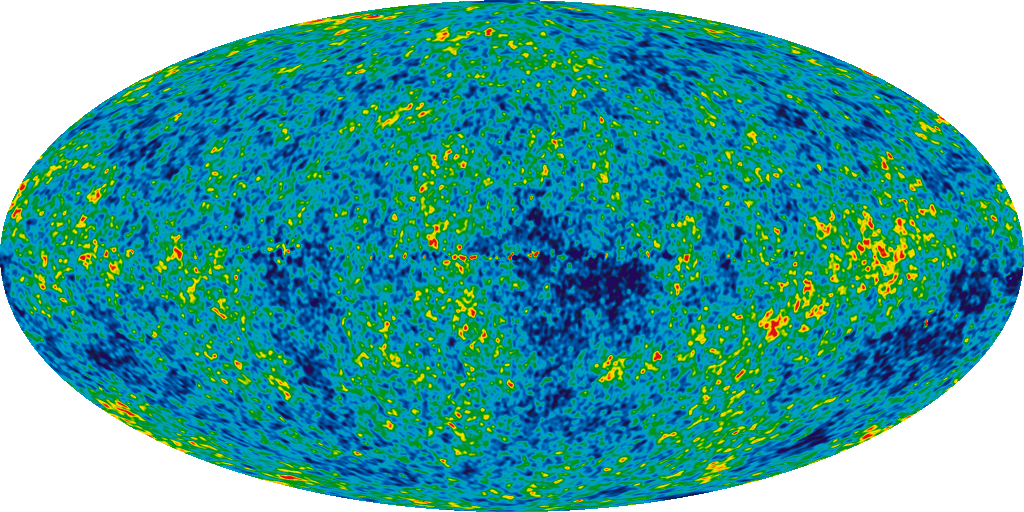
\includegraphics[width=\textwidth]{images/101080_7yrFullSky_WMAP_1024W.png}
\caption{The detailed, all-sky picture of the infant universe created from seven years of WMAP data. The image reveals 13.7 billion year old temperature fluctuations (shown as color differences) that correspond to the seeds that grew to become the galaxies. The signal from the our Galaxy was subtracted using the multi-frequency data. This image shows a temperature range of ± 200 microKelvin. Credit: NASA / WMAP Science Team}
\end{figure}

\item El otro gran descubrimiento en cosmología provino de la observación de que nuestro
universo se está expandiendo. Esto fue detectado inicialmente por Hubble (\citep{Hubble168}; \citep{hubblehumason1931}) basado en observaciones de variables cefeidas en varias nebulosas cercanas.

\begin{figure}[!h]
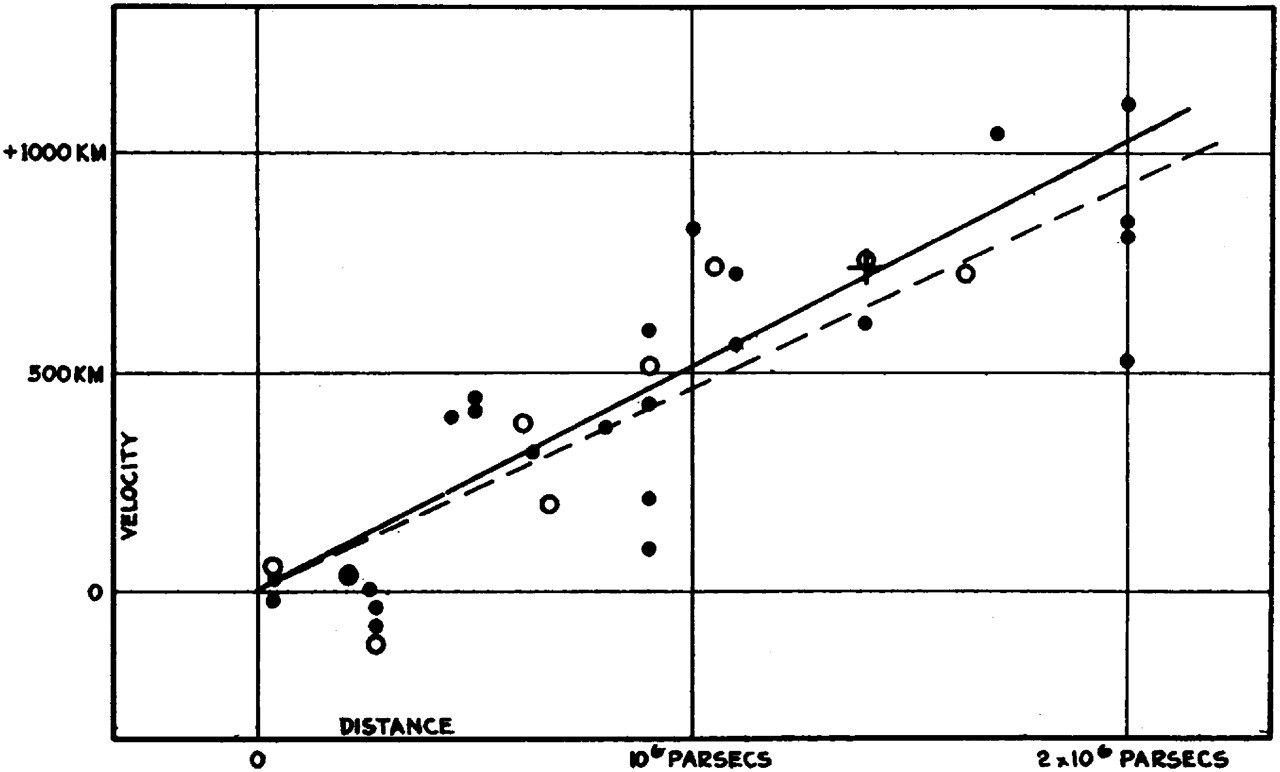
\includegraphics[width=\textwidth]{images/F2.large.jpg}
\caption{Hubble Law - Velocity-Distance Relation among Extra-Galactic Nebulae. Radial velocities, corrected for solar motion, are plotted against distances estimated from involved stars and mean luminosities of nebulae in a cluster. The black discs and full line represent the solution for solar motion using the nebulae individually; the circles and broken line represent the solution combining the nebulae into groups; the cross represents the mean velocity corresponding to the mean distance of 22 nebulae whose distances could not be estimated individually.}
\end{figure}

\end{itemize}


La expansión del Universo se ha confirmado a partir de observaciones de supernovas de tipo Ia (SNe
Ia)\footnote{SNe Ia son la fase explosiva de las enanas blancas que alcanzan el \Textit{límite de Chandrasekhar} despu\'es de acrecer masa de su compañero binario. Dadas las condiciones físicas de la explosión, la luminosidad producida
por la SN Ia se puede utilizar para medir la distancia a su galaxia anfitriona, raz\'on por la cual la SNs Ia se consideran como velas cosmológicas estándar.} (\citep{Riess_1998}; \citep{1999ApJ...517..565P}), que muestran que la expansión
en realidad, sucede a una tasa acelerada.  \\

Estos hechos implican que nuestro Universo era m\'as denso y caliente en el pasado (\Textit{Teor\'ia del Big Bang}). \\

La expansión del Universo est\'a asociada con la existencia de una energ\'ia de vac\'io,
generalmente referida como \Textit{Energía Oscura}. Según medidas de anisotrop\'ias del CMB ... \\